
\documentclass[14pt,aspectratio=169,notheorems]{beamer}

% Packages
% Shared content style for NN and NNDS. Written by Claude (2026-10-14).
%
% Everything that shared slides rely on lives here, loaded by both courses:
% colors, notation helpers and the card system. Course themes own only the
% presentation around the content (header, footer, title page, fonts, the
% \myalert color and where \SlideSource text goes). Change a definition here,
% never by redefining it in a course file, so the two courses cannot drift.

\usepackage{mathtools,amssymb,tcolorbox}
\tcbsetforeverylayer{autoparskip}

% Semantic colors
\definecolor{darkred}{rgb}{0.55,0,0}
\definecolor{darkpastelblue}{rgb}{0.47,0.62,0.8}
\definecolor{darkcerulean}{rgb}{0.03,0.27,0.49}
\definecolor{darkgreen}{rgb}{0,0.55,0}

% Figure palette (draw.io defaults)
\definecolor{titlecolor}{RGB}{245, 242, 238}
\definecolor{drawgray}{HTML}{666666}
\definecolor{drawgray_l}{HTML}{F5F5F5}
\definecolor{drawblue}{HTML}{6C8EBF}
\definecolor{drawblue_l}{HTML}{DAE8FC}
\definecolor{drawgreen}{HTML}{82B366}
\definecolor{drawgreen_l}{HTML}{D5E8D4}
\definecolor{draworange}{HTML}{D79B00}
\definecolor{draworange_l}{HTML}{FFE6CC}
\definecolor{drawyellow}{HTML}{D6B656}
\definecolor{drawyellow_l}{HTML}{FFF2CC}
\definecolor{drawred}{HTML}{B85450}
\definecolor{drawred_l}{HTML}{EA6B66}
\definecolor{drawviolet}{HTML}{9673A6}
\definecolor{drawviolet_l}{HTML}{E1D5E7}

% Notation
\newcommand{\vc}[1]{\boldsymbol{\mathbf{#1}}}
\DeclareMathOperator*{\argmax}{arg\,max}
\DeclareMathOperator*{\argmin}{arg\,min}

% Cards: blue for definitions and computable quantities, green for goals and
% stable formulations, orange for warnings and trade-offs, red for
% training-specific or problematic elements.
\tcbset{
	nndsblue/.style={colback=drawblue_l!35!white,colframe=drawblue,boxrule=0.8pt,arc=1mm},
	nndsgreen/.style={colback=drawgreen_l!35!white,colframe=drawgreen,boxrule=0.8pt,arc=1mm},
	nndsorange/.style={colback=draworange_l!35!white,colframe=draworange,boxrule=0.8pt,arc=1mm},
	nndsred/.style={colback=drawred_l!12!white,colframe=drawred,boxrule=0.8pt,arc=1mm}
}

% A card that opens with \[ would start with an empty paragraph line plus the
% display skip, leaving more room above than below (by an amount that differs
% between engines). Set that leading equation as a centered display-style line
% instead, so the space above it is the card padding, as below.
\makeatletter
\newcommand{\nndscardlead}{\futurelet\nndscard@next\nndscard@check}
% tcolorbox follows this hook with \ignorespaces; look past it.
\def\nndscard@check{\ifx\nndscard@next\ignorespaces
	\expandafter\nndscard@skip\else\expandafter\nndscard@test\fi}
\def\nndscard@skip\ignorespaces{\nndscard@test}
\newcommand{\nndscard@test}{\@ifnextchar\[{\nndscard@display}{}}
\def\nndscard@display\[#1\]{{\centering$\displaystyle#1$\par}\@ifnextchar\end{}{\vspace{\belowdisplayskip}}}
\makeatother

% Card text is ragged-right: narrow justified columns open wide word gaps,
% especially in NNDS, which never hyphenates. Fixed display spacing: when
% parallel cards share a height, stretchable skips would otherwise spread
% the content unevenly.
\tcbset{
	nndscard/.style={before upper={\raggedright
		\setlength{\abovedisplayskip}{6pt}\setlength{\belowdisplayskip}{6pt}%
		\setlength{\abovedisplayshortskip}{6pt}\setlength{\belowdisplayshortskip}{6pt}%
		\nndscardlead}},
	nndsblue/.append style={nndscard},
	nndsgreen/.append style={nndscard},
	nndsorange/.append style={nndscard},
	nndsred/.append style={nndscard}
}

% Parallel cards share a group name and get equal heights; the second argument
% (a fixed height used by older NNDS slides) is ignored.
\tcbset{courseheight/.style 2 args={equal height group=#1}}

\usepackage{tikz}

% Matrix shapes written under a symbol, e.g. \shape{\vc{Q}}{(T,D_k)}.
\usepackage{stackengine}
\stackMath
\def\sss{\scriptstyle \color{gray}}
\setstackgap{L}{12pt}
\def\stacktype{L}
\newcommand{\shape}[2]{\stackunder{#1}{\sss #2}}

% Transformer slides: colors and diagram styles (moved here from the NNDS
% transformers-settings.tex on 2026-11-16, when NN adopted the lecture).

% Query, key and value colors, reused in equations and figures.
\colorlet{qcolor}{drawviolet!80!black}
\colorlet{kcolor}{draworange!85!black}
\colorlet{vcolor}{darkcerulean}
\newcommand{\qc}[1]{{\color{qcolor}#1}}
\newcommand{\kc}[1]{{\color{kcolor}#1}}
\newcommand{\vcl}[1]{{\color{vcolor}#1}}

% Block-diagram styles, as in shared/slides/mlps.tex and the deeper-models deck.
\tikzset{
    nnblock/.style={
            draw=drawblue, fill=drawblue_l!25!white, rounded corners=2pt,
            minimum width=1.25cm, minimum height=0.65cm,
            inner sep=5pt, font=\small
        },
    nnother/.style={nnblock, draw=drawgreen, fill=drawgreen_l!25!white},
    nnmerge/.style={
            circle, draw=drawgray, fill=white,
            minimum size=0.55cm, inner sep=1pt, font=\small
        },
    nnedge/.style={->, thick, draw=drawgray}
}

% Full-size diagram styles for the transformer figures: arrows as in the
% attention figures (Stealth tips, gray), boxes at normal size.
\tikzset{
    tfarr/.style={-{Stealth[length=5pt]}, drawgray, line width=0.6pt},
    tfblk/.style={draw=drawblue, fill=drawblue_l!60, rounded corners=2pt,
            minimum height=0.75cm, minimum width=1.9cm, inner sep=4pt, font=\small},
    tfnorm/.style={tfblk, draw=drawgreen, fill=drawgreen_l!70},
    tfsum/.style={circle, draw=drawgray, fill=white, minimum size=0.45cm, inner sep=0pt, font=\small},
    tflab/.style={font=\scriptsize, text=black!60},
}

\usepackage{mathtools}
\usepackage{hyperref}
\usepackage{setspace}
\usepackage{tikz}
\usetikzlibrary{positioning}
\usepackage{ragged2e}
\usepackage{nicematrix}
\usepackage[compatibility=false]{caption}
\usepackage[framemethod=tikz]{mdframed}


% Theme
\usetheme{metropolis}
\metroset{subsectionpage=progressbar,sectionpage=none}
\setbeamertemplate{theorems}[numbered]

\usepackage{fontspec}
\defaultfontfeatures{LetterSpace=30}
\usepackage{microtype}

% Prefer flexible inter-word spacing over splitting words across lines.
\tolerance=1
\emergencystretch=\maxdimen
\hyphenpenalty=10000
\hbadness=10000


% Code
\usepackage{listings}
% Custom colors
\definecolor{codegreen}{rgb}{0,0.6,0}
\definecolor{codegray}{rgb}{0.5,0.5,0.5}
\definecolor{codepurple}{rgb}{0.58,0,0.82}
\definecolor{backcolour}{rgb}{0.95,0.95,0.92}
\definecolor{light-gray}{gray}{0.95}
% Python style for highlighting
\newcommand\pythonstyle{\lstset{
		backgroundcolor=\color{white},
		language=Python,
		basicstyle=\ttfamily\footnotesize,
		morekeywords={self},              % Add keywords here
		keywordstyle=\color{blue},
		stringstyle=\footnotesize\color{deepgreen},
		commentstyle=\color{codegreen},
		showstringspaces=false,
		frame=tb,
		numbers=left,
		numbersep=5pt,
		numberstyle=\tiny\color{gray},
		columns=fullflexible,
		numbersep=5pt,
		aboveskip=1em,
		showtabs=false,
		tabsize=2,
		gobble=3
	}}

% Python environment
\lstnewenvironment{python}[1][]
{
	\pythonstyle
	\lstset{#1}
}
{}
% Python for inline
\newcommand\pythoninline[1]{{\pythonstyle\lstinline!#1!}}

% Tables and justification
\newcommand{\ra}[1]{\renewcommand{\arraystretch}{#1}}
\justifying

% Subfigures
\setbeamertemplate{caption}[numbered]
\usepackage[caption=false,font=footnotesize]{subfig}

% Colors
\setbeamercolor{uppercolgreen}{fg=white,bg=green!35}
\setbeamercolor{lowercolgreen}{fg=black,bg=green!10}
\setbeamercolor{uppercolred}{fg=white,bg=red!35}
\setbeamercolor{lowercolred}{fg=black,bg=red!10}
\setbeamercolor{uppercolblue}{fg=white,bg=blue!35}
\setbeamercolor{lowercolblue}{fg=black,bg=blue!10}
\definecolor{deepblue}{rgb}{0,0,0.5}
\definecolor{deepred}{rgb}{0.6,0,0}
\definecolor{deepgreen}{rgb}{0,0.5,0}

% Mathematical commands
\newcommand{\pr}[1]{{#1\,}'}
\newcommand{\idx}[2]{{\color{darkpastelblue}[}#1{\color{darkpastelblue}]_{#2}}}
% Course switch for shared slides: \NNDSorNN{NNDS text}{NN text}.
\newcommand{\NNDSorNN}[2]{#1}

% Style commands
\newcommand{\myalert}[1]{{\color{darkred}\textbf{#1}}}

% White background on every slide, so figures with a white canvas blend in
% (Simone, 2026-10-14). whiteframe is kept as an alias for existing slides.
\setbeamercolor{background canvas}{bg=white}

% White frame (for images)
\newenvironment{whiteframe}[1]{
	\setbeamercolor{background canvas}{bg=white}
	\begin{frame}{#1}
		}{
	\end{frame}
}

\setbeamerfont{frametitle}{size=\normalsize}
\setbeamertemplate{frametitle}[default][right]
% Slimmer header, close to NN's share of the slide height (Simone, 2026-10-14).
\makeatletter
\patchcmd{\beamer@@tmpl@frametitle}{sep=0.3cm}{sep=0.2cm}{}{\PackageWarning{style}{frametitle padding not patched}}
\makeatother
{
}
%\setbeamercolor{frametitle}{fg=white,bg=black!75}

% No headline frame
\makeatletter
\newenvironment{noheadline}{
	\setbeamertemplate{headline}{}
	\addtobeamertemplate{frametitle}{\vspace*{-3.5\baselineskip}}{}
}{}
\makeatother

% Lists
\setbeamertemplate{itemize items}[triangle]

% Footnotes
\setbeamertemplate{footnote}%
{%
	\parindent 1.5em\noindent%
	\justifying\setstretch{0.7}%
	\hbox to 1em{\hfil\insertfootnotemark}\begin{scriptsize}\insertfootnotetext\end{scriptsize}\par%
}

% Footnote without number
\newcommand\blfootnote[1]{%
	\begingroup
	\renewcommand\thefootnote{}\footnote[frame]{\noindent#1}%
	\addtocounter{footnote}{-1}%
	\endgroup
}

% Slide sources: set in the frame footer beside the page number, so they
% take no room from the content. Zero height keeps the footline unchanged.
% Global, because the footline is typeset outside the frame's group; each
% frame starts empty.
\newcommand{\insertslidesource}{}
\newcommand{\SlideSource}[1]{\gdef\insertslidesource{#1}}
\AddToHook{env/frame/begin}{\gdef\insertslidesource{}}
\setbeamertemplate{frame footer}{%
	\ifx\insertslidesource\empty\else
		\smash{\parbox[b]{0.88\textwidth}{\raggedright\scriptsize\color{black!60}\insertslidesource}}%
	\fi}

% Theorems
\newcommand*{\theorembreak}{\usebeamertemplate{theorem end}\framebreak\usebeamertemplate{theorem begin}}
\newcounter{theo}[section]\setcounter{theo}{0}
\renewcommand{\thetheo}{\arabic{section}.\arabic{theo}}

\newenvironment{theo}[2][]{%
	\refstepcounter{theo}%
	\ifstrempty{#1}%
	{\mdfsetup{%
			frametitle={%
					\tikz[baseline=(current bounding box.east),outer sep=0pt]
					\node[anchor=east,rectangle,fill=red!10]
					{\strut Theorem~\thetheo};}}
	}%
	{\mdfsetup{%
			frametitle={%
					\tikz[baseline=(current bounding box.east),outer sep=0pt]
					\node[anchor=east,rectangle,fill=red!10]
					{\strut Theorem~\thetheo:~#1};}}%
	}%
	\mdfsetup{innertopmargin=5pt,linecolor=red!10,%
		linewidth=2pt,topline=true,%
		frametitleaboveskip=\dimexpr-\ht\strutbox\relax
	}
	\begin{mdframed}[]\relax%
		\label{#2}}{\end{mdframed}}

\setbeamerfont{frametitle}{size=\large}

\graphicspath{{assets/}{../../shared/assets/}}
\begin{document}

{\usebackgroundtemplate{\tikz\node[opacity=0.4,inner sep=0]{
\includegraphics[width=\paperwidth,height=\paperheight]{images/header}};}%
\begin{frame}[plain]
	\vspace{0.5cm}
	\title{\large \begin{spacing}{1.0}Neural Networks for Data Science\end{spacing}\vspace{0.25em}
		\normalsize \begin{spacing}{1.0}\textbf{Master's Degree in Data Science}\end{spacing}\vspace{0.5em}}
	\subtitle{\Large \textbf{Lecture 0: About the course}}
	\date{
		{
\includegraphics[scale=0.8]{images/Uniroma1}}
	}
	\author{
		\setlength{\tabcolsep}{2pt}
		\begin{tabular}{rl}
			\textbf{Lecturer}: & S. Scardapane \\
		\end{tabular}
	}\titlepage
\end{frame}
}

\part{1}

\begin{frame}{Before we start}

	\begin{itemize}
		\item \textbf{Master's Degree in Data Science}, code 10589627, 2nd year, optional group D.
		\item \textbf{Timetable}: Thursdays 09:00--12:00 and Fridays 09:00--11:00, room A5 (Via Ariosto), 24 September -- 18 December 2026.
		\item \textbf{Office hours}: by appointment, remotely or in person.
	\end{itemize}

	\begin{tcolorbox}
		\href{https://www.sscardapane.it/teaching/nnds-2026/}{https://www.sscardapane.it/teaching/nnds-2026/}
	\end{tcolorbox}

	Register for \textbf{Google Classroom} from the website: it is mandatory for receiving announcements.

\end{frame}

\begin{frame}{Exam dates (2027)}

	\begin{itemize}
		\item \textbf{Sessions 1--2}: 13 January, 3 February.
		\item \textbf{Sessions 3--4}: 16 June, 14 July.
		\item \textbf{Session 5}: 15 September.
		\item \textbf{Extraordinary E1}: 7 April.
		\item \textbf{Extraordinary E2}: 13 October.
	\end{itemize}

\end{frame}

\begin{frame}{Oral exam}
	\small

	The default exam is an \textbf{oral examination}, usually with one or two questions.

	\begin{itemize}
		\item Define a concept such as dropout. Give core definitions with the same mathematical detail as in the slides.
		\item Reason about a layer, for example by working out its output shape or explaining the effect of a hyperparameter.
	\end{itemize}

	Questions cover lecture material taught in class. Labs, coding exercises and topics skipped in class are outside the scope. If you are unsure about a topic, ask me before the exam.

\end{frame}

\begin{frame}{Research project: getting started}
	\small

	An individually approved \textbf{research project and defense} can replace the oral if you are aiming for \textbf{30 e lode} or preparing for a follow-up \textbf{thesis}. Plan for about one month of work.

	\begin{itemize}
		\item Contact me at any time if you want to propose an idea or ask for a topic.
		\item We start with a short interview. I check your preparation at the same level as the oral exam, and we discuss possible topics.
		\item Before starting, we agree on a short outline: the research question, what it adds to the closest prior work, and what evidence would answer it.
	\end{itemize}

\end{frame}

\begin{frame}{Research project: evidence and review}
	\small

	The project must answer the agreed question. A well-supported negative result is valid. For example, a fair comparison can show that a proposed change gives no improvement under the conditions we agreed to test.

	\begin{itemize}
		\item Once you have preliminary results, we use an AI-assisted review to check the comparisons, controls and conclusions. We may do a second pass if major issues remain.
		\item Explain briefly how you addressed the main review comments. You can use AI tools in the project. In your report, say where they made a substantial contribution and how you checked their output.
	\end{itemize}

\end{frame}

\begin{frame}{Research project: submission and defense}
	\small

	\begin{itemize}
	\item Submit a short report and, where applicable, the code and instructions needed to reproduce the main result. Agree with me on your session and how and when to submit.
	\item Project defenses are grouped with the oral exams during the regular exam sessions. You give a short presentation and answer questions about your choices and results.
	\item I grade the project and defense on the usual exam scale. If the evidence leaves the question open, we may agree on a focused revision. The oral is the fallback for an incomplete project.
	\end{itemize}

\end{frame}

\begin{frame}{The course in one slide}

	\begin{enumerate}
		\item \textbf{Fundamentals}\\
		      Arrays, optimization, supervised learning, MLPs, automatic differentiation, and PyTorch (maybe JAX).
		\item \textbf{Architectures}\\
		      Images, sequences, text, and graphs; convolutions, recurrence, attention, and message passing.
		\item \textbf{Applications}\\
		      Tokenization, pre- and post-training, self-supervised learning, possibly agents.
	\end{enumerate}

\end{frame}

\begin{whiteframe}{Alice in a {\color{yellow}differentiable} wonderland}


	Slides are self-contained, but most of the material is expanded in a textbook:

	\vspace{1em}
	\begin{columns}
		\begin{column}{0.25\textwidth}
			\begin{center}
				{%
					\setlength{\fboxsep}{0pt}%
					\setlength{\fboxrule}{1pt}%
					\fbox{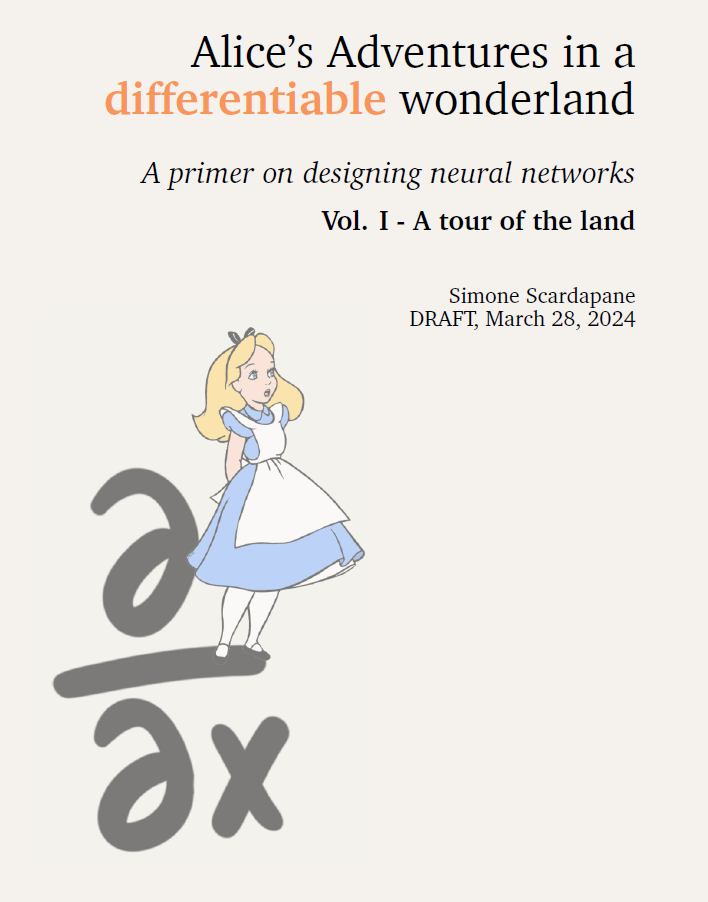
\includegraphics[width=0.2\pagewidth]{images/Alice.png} }%
				}%
			\end{center}
		\end{column}
		\begin{column}{0.75\textwidth}
			The book is available for free as a PDF or as a printed copy:

			\begin{center}\footnotesize\url{https://sscardapane.it/alice-book/}\end{center}

			You can also find additional lab sessions and chapters (e.g., more on post-training of models and automatic differentiation).
		\end{column}
	\end{columns}



\end{whiteframe}

{\setbeamercolor{background canvas}{bg=light-gray}
\begin{frame}{Structured Neural Intelligence Lab}
	\begin{center}
		{\setlength{\fboxsep}{0pt}\setlength{\fboxrule}{1.25pt}%
			\color{darkcerulean}\href{https://www.sscardapane.it/snail/}{\fbox{
\includegraphics[width=0.70\paperwidth]{images/SNAIL_homepage.png}}}}\\[0.4em]
		\small Explore the group: \href{https://www.sscardapane.it/snail/}{www.sscardapane.it/snail}
	\end{center}
\end{frame}
}

\begin{whiteframe}{Optional resource: TinyTorch}
	\begin{columns}[T,onlytextwidth]
		\begin{column}{0.32\textwidth}
			\vspace{0.25em}
			\small
			\textbf{A hands-on implementation of PyTorch from scratch.}

			\vspace{0.5em}
			More in-depth than our lab sessions. Let me know if you try them.

			\scriptsize Disclaimer: I have not.

			\vspace{0.5em}
			\scriptsize\url{https://mlsysbook.ai/tinytorch/}
		\end{column}
		\begin{column}{0.66\textwidth}
			\centering
			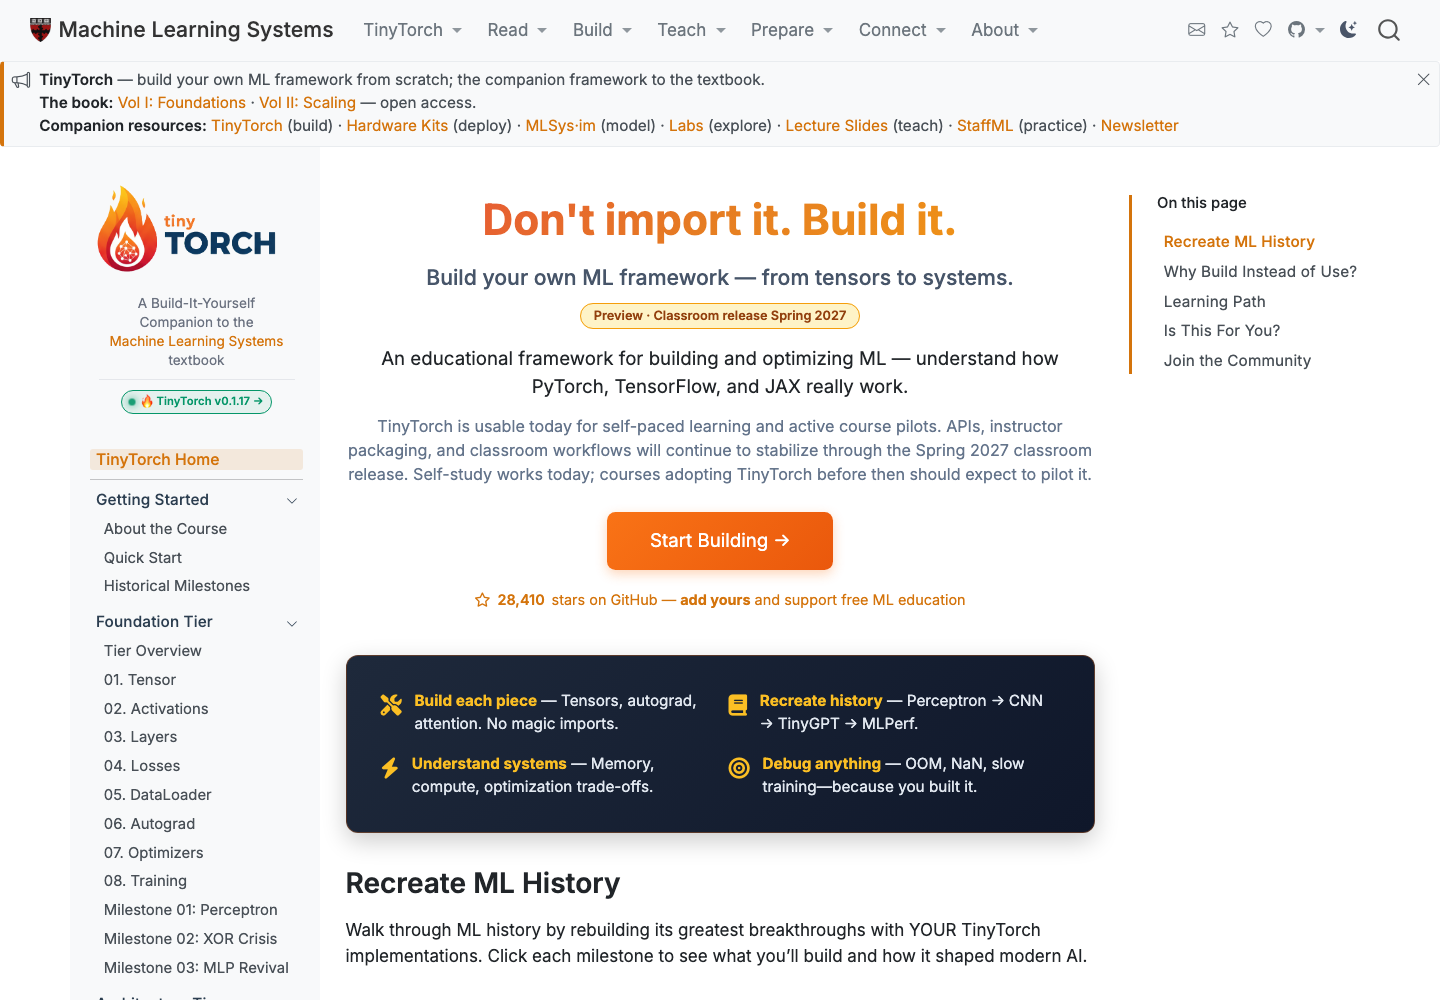
\includegraphics[height=0.48\textheight,keepaspectratio]{images/TinyTorch.png}
		\end{column}
	\end{columns}
\end{whiteframe}

\end{document}
